\section{Setting up the Scilab software}

	\subsection{Installing Scilab}
		\begin{enumerate}[I.]
			\item Visit the download page of Scilab available at: \url{https://www.scilab.org/download/}
			\begin{figure}[h!]
				\centering
				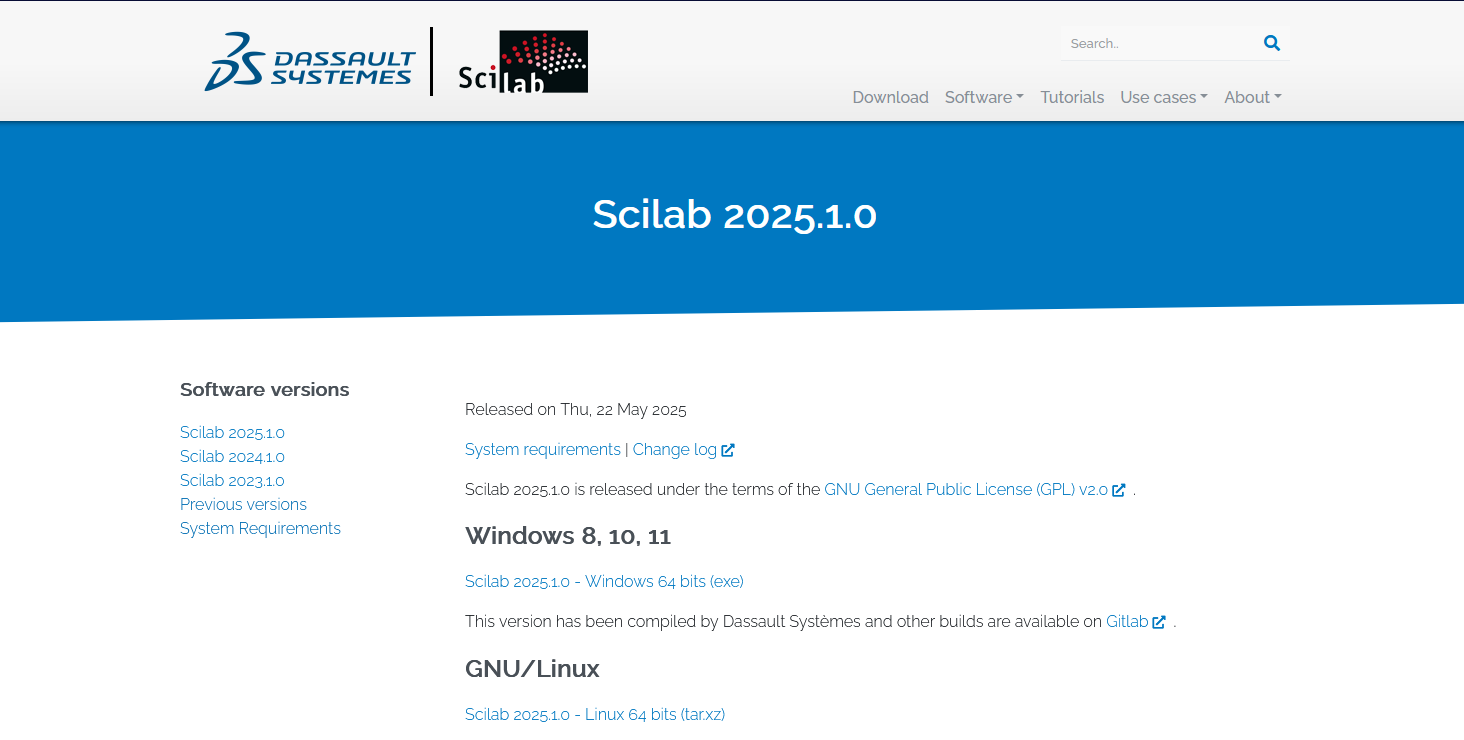
\includegraphics[width=0.5\linewidth,frame]{figures/fig_scilab-download-page.png}
				\caption{The webpage for downloading the latest version of Scilab}
				\label{fig:scilab-download}
			\end{figure}
			
			\item Click on the relevant link to download Scilab for Windows, Linux or MacOS.
			
			\item Navigate to the folder containing the downloaded file and install the software on the PC. Select `English' as the preferred language the then click on `OK' to proceed with the rest of the installation process as illustrated below:
			\begin{figure}[!htb]
				\centering
				\begin{subfigure}[b]{0.3\textwidth}
					\centering
					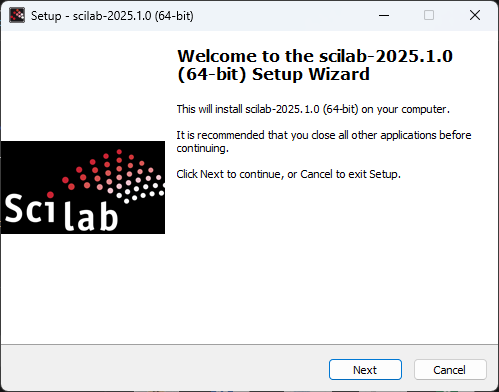
\includegraphics[width=\textwidth,frame]{figures/installation/fig_installation-02.png}
					% \caption{$y=x$}
				\end{subfigure}
				\hfill
				\begin{subfigure}[b]{0.3\textwidth}
					\centering
					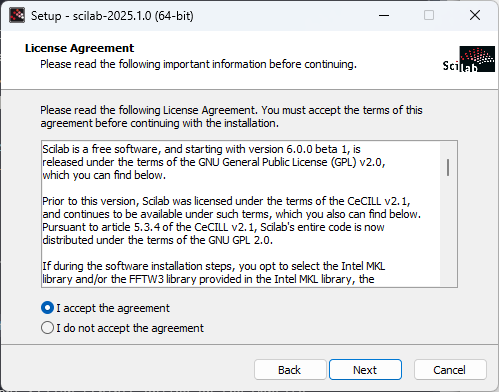
\includegraphics[width=\textwidth,frame]{figures/installation/fig_installation-03.png}
					% \caption{$y=x$}
				\end{subfigure}
				\hfill
				\begin{subfigure}[b]{0.3\textwidth}
					\centering
					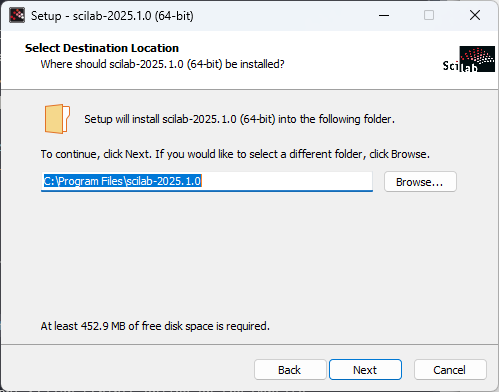
\includegraphics[width=\textwidth,frame]{figures/installation/fig_installation-04.png}
					% \caption{$y=x$}
				\end{subfigure}
				
				\vspace{0.2cm}
				\begin{subfigure}[b]{0.3\textwidth}
					\centering
					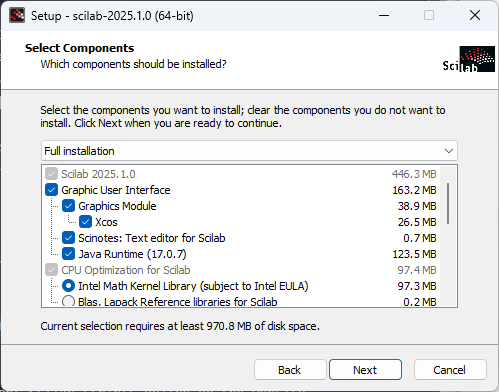
\includegraphics[width=\textwidth,frame]{figures/installation/fig_installation-05.png}
					% \caption{$y=x$}
				\end{subfigure}
				\hfill
				\begin{subfigure}[b]{0.3\textwidth}
					\centering
					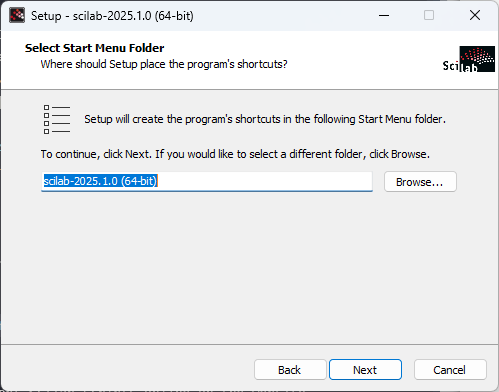
\includegraphics[width=\textwidth,frame]{figures/installation/fig_installation-06.png}
					% \caption{$y=x$}
				\end{subfigure}
				\hfill
				\begin{subfigure}[b]{0.3\textwidth}
					\centering
					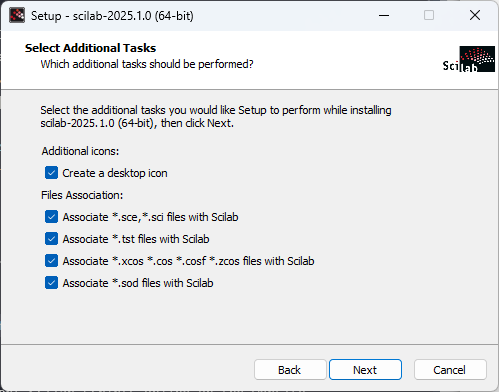
\includegraphics[width=\textwidth,frame]{figures/installation/fig_installation-07.png}
					% \caption{$y=x$}
				\end{subfigure}
				
				\vspace{0.2cm}
				\begin{subfigure}[b]{0.3\textwidth}
					\centering
					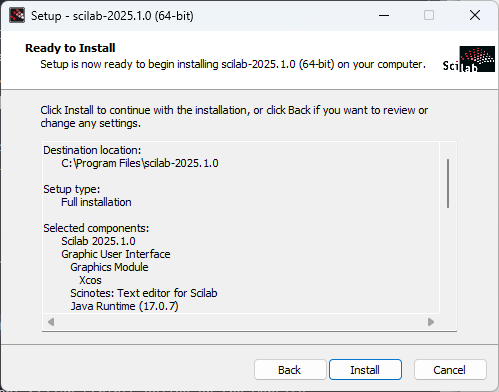
\includegraphics[width=\textwidth,frame]{figures/installation/fig_installation-08.png}
					% \caption{$y=x$}
				\end{subfigure}
				\hfill
				\begin{subfigure}[b]{0.3\textwidth}
					\centering
					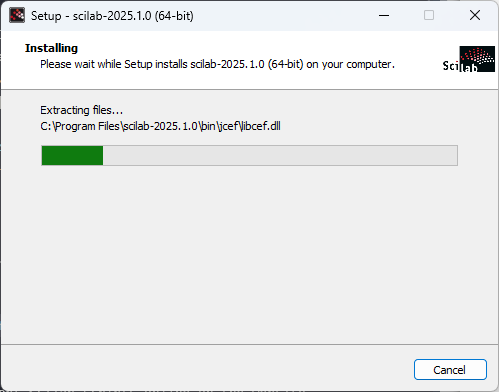
\includegraphics[width=\textwidth,frame]{figures/installation/fig_installation-09.png}
					% \caption{$y=x$}
				\end{subfigure}
				\hfill
				\begin{subfigure}[b]{0.3\textwidth}
					\centering
					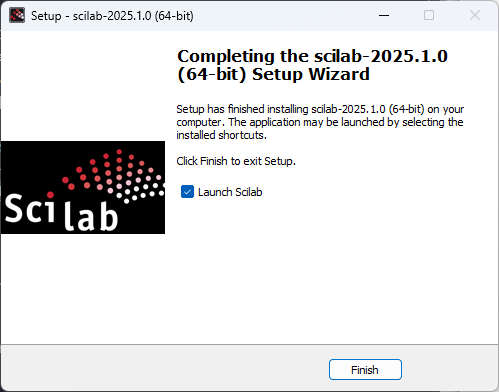
\includegraphics[width=\textwidth,frame]{figures/installation/fig_installation-10.png}
					% \caption{$y=x$}
				\end{subfigure}
			\end{figure}
		\end{enumerate}
	
	\subsection{Scilab on Cloud}
		The \textit{National Virtual Library of India}\footnote{\url{https://www.rrrlf.gov.in/NML/NVLI.aspx}} maintains an online version of Scilab on the Garuda Cloud. This is known as \textit{Scilab on Cloud} and is available at:
		\url{https://cloud.scilab.in/}
		
		The online interface of \textit{Scilab on Cloud} is displayed in figure \ref{fig:cloud-scilab}.
		\begin{figure}[!htb]
			\centering
			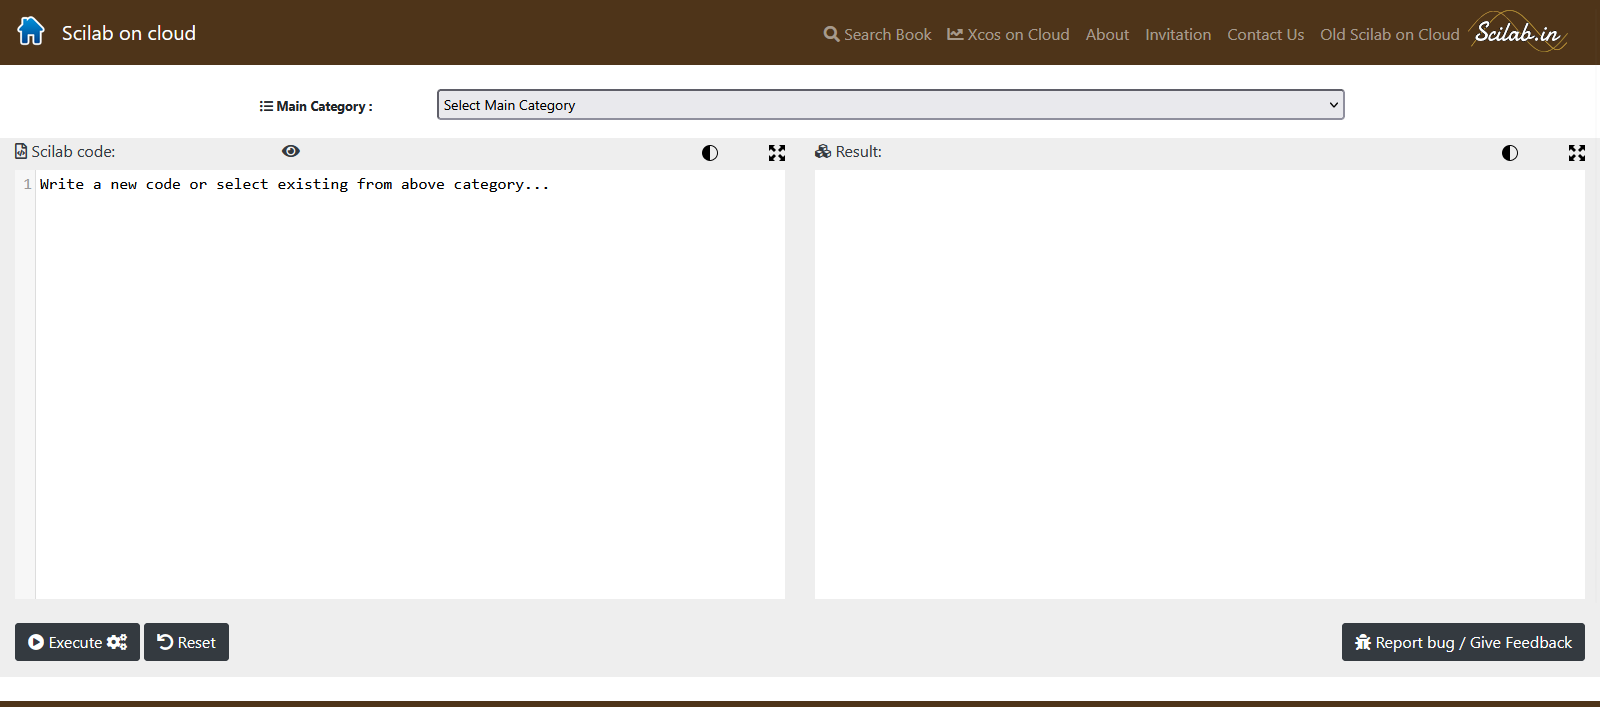
\includegraphics[width=0.7\textwidth,frame]{figures/fig_cloud-scilab.png}
			\caption{Scilab on Cloud}
			\label{fig:cloud-scilab}
		\end{figure}
		
		One can type the Scilab code on the left panel, then click on `Execute' to view the output on the right panel.
	
	\subsection{Launching Scilab}
		One can find the Scilab icon on the desktop or in the list of installed applications on one's PC. Simply clicking on the icon launches Scilab with its default GUI which is displayed in figure \ref{fig:default-gui} below.
		
		\begin{figure}[!htb]
			\centering
			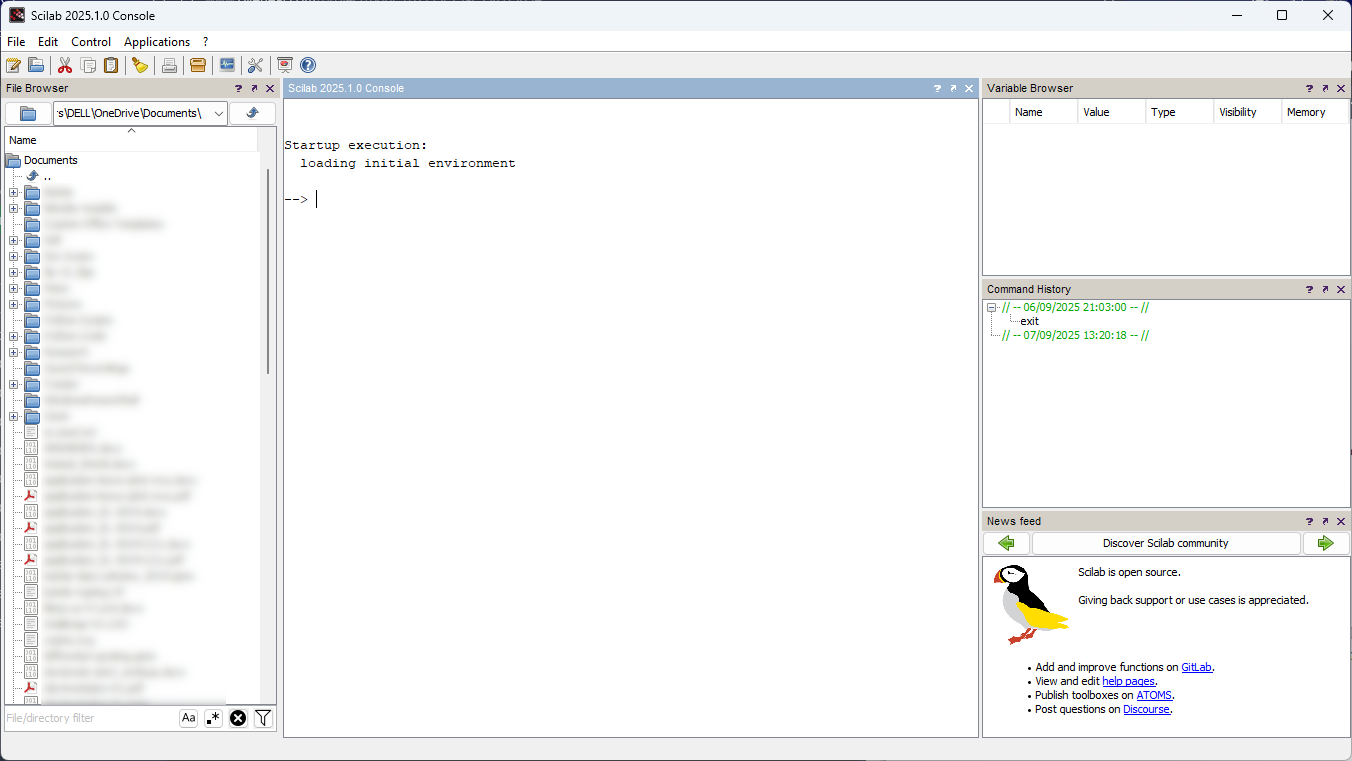
\includegraphics[width=0.8\textwidth,frame]{figures/gui/fig_default-gui.png}
			\caption{Default graphical user interface (GUI) of Scilab}
			\label{fig:default-gui}
		\end{figure}